\documentclass[12pt,openright,twoside,french]{book}

\input philippe2013
\input philippe2013_activites
\pagestyle{empty}


\begin{document}

\TitreActivite{vii.3}{Qu'est ce que le \\ produit scalaire ?}

En mécanique, une force s'appliquant en un point est représentée par un vecteur dont la norme est proportionnelle à l'intensité de la force exprimée en Newton.\medskip

\exo

Sur les schémas ci-dessous, le mobile rectangulaire se déplace toujours suivant le vecteur $\vect{AB}$. On lui applique une force $\vect F$ au point $A$. Quel semble être l'effet de cette force sur le déplacement du mobile ?

\begin{center}
    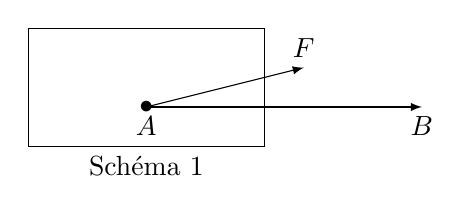
\begin{tikzpicture}[scale=0.5,>=latex]
        \draw (0,0) rectangle (6,3);
        \draw[->] (3,1) node[below] {$A$} node {$\bullet$} -- (10,1) node[below] {$B$};
        \draw[->] (3,1) -- (7,2) node[above] {$\vect F$};
        \draw(3,0) node[below] {Schéma $1$};
    \end{tikzpicture}\qquad
    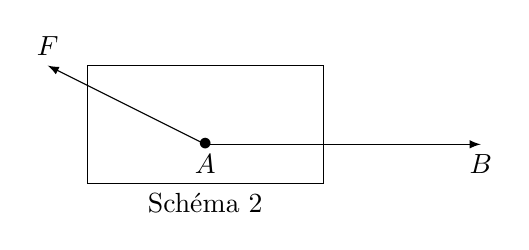
\begin{tikzpicture}[scale=0.5,>=latex]
        \draw (0,0) rectangle (6,3);
        \draw[->] (3,1) node[below] {$A$} node {$\bullet$} -- (10,1) node[below] {$B$};
        \draw[->] (3,1) -- (-1,3) node[above] {$\vect F$};
        \draw(3,0) node[below] {Schéma $2$};
    \end{tikzpicture}\qquad
    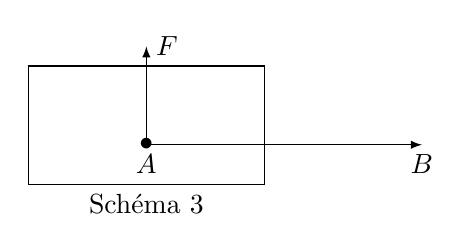
\begin{tikzpicture}[scale=0.5,>=latex]
        \draw (0,0) rectangle (6,3);
        \draw[->] (3,1) node[below] {$A$} node {$\bullet$} -- (10,1) node[below] {$B$};
        \draw[->] (3,1) -- (3,3.5) node[right] {$\vect F$};
        \draw(3,0) node[below] {Schéma $3$};
    \end{tikzpicture}
\end{center}\medskip

\exo

On considère 2 forces $\vect{F_1}$ et $\vect{F_2}$ s'appliquant en un point $O$ telles que l'angle $\left(\vect{F_1} , \vect{F_2}\right)$ ait pour mesure $\alpha$.\par
La force résultante $\vect{R}$ est égale à $\vect{R} = \vect{F_1} + \vect{F_2}$.\par

On prend $\norme{\vect{F_1}} = F_1 = 10 N$, $\norme{\vect{F_2}} = F_2 = 50 N$ et $\alpha = \frac\pi 6$.\medskip

\begin{enumerate}
    \item \textbf{Graphiquement.}\par
        En prenant pour unité graphique $1~cm$ pour $10 N$, représenter les forces $\vect{F_1}$, $\vect{F_2}$ et $\vect{R}$.\par
        En mesurant sur la représentation, donner une valeur approchée de l'intensité de la résultante.
    \item \textbf{Dans un repère.}\par
        On considère le repère orthonormal $\Oij$ tel que le vecteur $\vect\imath$ ait la même direction et le même sens que la force $\vect{F_1}$.
        \begin{enumerate}
            \item Faire une figure et construire la force résultante $\vect{R}$.
            \item \'Ecrire les coordonnées de \vect{F_1} en fonction de $F_1$.
            \item \'Ecrire les coordonnées de \vect{F_2} en fonction de $F_2$ et $\alpha$.
            \item \'Ecrire les coordonnées de \vect{R}.
            \item \'Etablir la relation suivante $R^2 = F_1^2 + F_2^2 + 2F_1F_2cos \alpha$.
            \item Calculer alors l'intensité de la résultante pour les valeurs numériques données de $F_1$, $F_2$ et $\alpha$.
        \end{enumerate}
\end{enumerate}\bigskip

Le nombre $F_1F_2 cos \alpha$ est appelé produit scalaire des vecteurs \vect{F_1} et \vect{F_2}.


\end{document} 